\section{Moore's Law}

\qcontributor{Regina Eckert}

Moore's Law is a 1965 observation by Fairchild Semiconductor Research and Development Lab's director, Gordon Moore, that the number of transistors on an integrated circuit chip doubles every 1.5-2 years. This observation has dominated the computer industry into modern day, where we now have sophisticated processes to create transistors that have a smallest feature size that is 10 \si{\nano\meter} across.

\iffalse
	\begin{figure}[H]{
		\centering
		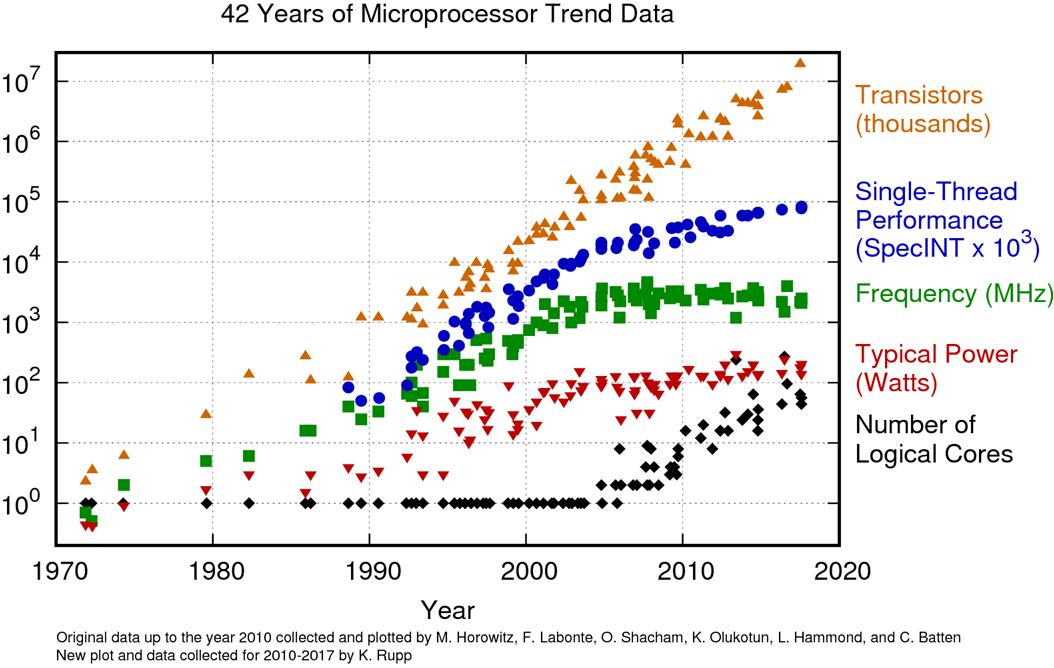
\includegraphics[width=0.8\textwidth]{n_moores_law/moores_law.png}
		\caption{Result of Moore's Law from 1970 to present day}
		\vspace{-5mm}}
	\label{fig:Moores}
\end{figure}

Figure source: https://www.karlrupp.net/.
\fi